\documentclass[conf]{new-aiaa} % Use [journal] for AIAA journal style

%\usepackage[utf8]{inputenc}

%graphics packages
\usepackage[]{graphicx}
\graphicspath{{./figures/}}

% ------------------ tikz ------------
%%tikz
\RequirePackage{pgf,tikz}
\usepackage{pgfplots}
\pgfplotsset{compat=newest}
\usetikzlibrary{arrows.meta}
\usetikzlibrary{arrows}
\usetikzlibrary{shapes.geometric}
\usetikzlibrary{shapes.misc}
\usetikzlibrary{backgrounds}
\usetikzlibrary{bending}
\usetikzlibrary{shadows}
\usetikzlibrary{patterns}
\usetikzlibrary{patterns.meta}
\usetikzlibrary{intersections}
\usepgfplotslibrary{patchplots}
\usepgfplotslibrary{fillbetween}
\usepgfplotslibrary{groupplots}
\usepgfplotslibrary{polar}
\usepgfplotslibrary{smithchart}
\usepgfplotslibrary{statistics}
\usepgfplotslibrary{dateplot}
\usepgfplotslibrary{ternary}
\pgfplotsset{%
	layers/standard/.define layer set={%
		background,axis background,axis grid,axis ticks,axis lines,axis tick labels,pre main,main,axis descriptions,axis foreground%
	}{grid style= {/pgfplots/on layer=axis grid},%
		tick style= {/pgfplots/on layer=axis ticks},%
		axis line style= {/pgfplots/on layer=axis lines},%
		label style= {/pgfplots/on layer=axis descriptions},%
		legend style= {/pgfplots/on layer=axis descriptions},%
		title style= {/pgfplots/on layer=axis descriptions},%
		colorbar style= {/pgfplots/on layer=axis descriptions},%
		ticklabel style= {/pgfplots/on layer=axis tick labels},%
		axis background@ style={/pgfplots/on layer=axis background},%
		3d box foreground style={/pgfplots/on layer=axis foreground},%
	},
}
% new style at automates partial ellipse
\tikzset{
    partial ellipse/.style args={#1:#2:#3}{
        insert path={+ (#1:#3) arc (#1:#2:#3)}
    }
}

\usepackage{caption}
\usepackage{subcaption}
\usepackage{placeins}
\usepackage{wrapfig}
\usepackage{url}

%tables
\usepackage{array}
\newcommand{\PreserveBackslash}[1]{\let\temp=\\#1\let\\=\temp}
\newcolumntype{C}[1]{>{\PreserveBackslash\centering}m{#1}}
\newcolumntype{R}[1]{>{\PreserveBackslash\raggedleft}m{#1}}
\newcolumntype{L}[1]{>{\PreserveBackslash\raggedright}m{#1}}

%mathpackages
\usepackage{amsmath}
%\usepackage{siunitx}
%\usepackage{mathrsfs}
%\newcommand{\vect}{\overset{\rightharpoonup}}
%decrease overset height
% \makeatletter
% \newcommand{\oset}[3][0.25ex]{%
% 	\mathrel{\mathop{#3}\limits^{
% 			\vbox to#1{\kern-0.5\ex@
% 				\hbox{$\scriptstyle#2$}\vss}}}}
% \makeatother

%%Vector arrow over variable
%\newcommand{\vect}[1]{%
%	\oset{\rightharpoonup}{#1}}

\RequirePackage{bm}
\newcommand{\vect}[1]{\bm{#1}}

\newcommand{\mat}[1]{%
	\mathbf{#1}}
\usepackage{nicefrac}
\usepackage{cancel}

%referencing packages
\usepackage{hyperref}
\usepackage[]{cleveref}

% ---------- colors -------------
\RequirePackage{xcolor}
\definecolor{navy}{HTML}{002E5D}
\definecolor{royal}{HTML}{005CAB}	% royal that matches BYU Engineering logo
\definecolor{darkgray}{HTML}{141414}
\definecolor{mediumgray}{HTML}{666666}	% medium gray definition from A. Ning
\definecolor{black}{HTML}{111111}
\definecolor{primary}{HTML}{005CAB}
\definecolor{secondary}{HTML}{c05367}
\definecolor{tertiary}{HTML}{8fa651}
\definecolor{plotsgray}{HTML}{808080}


% -------------- easy coloring of things ----------------
\newcommand{\navy}[1]{{\color{navy}#1}}
\newcommand{\primary}[1]{{\color{primary}#1}}
\newcommand{\secondary}[1]{{\color{secondary}#1}}
\newcommand{\tertiary}[1]{{\color{tertiary}#1}}
\newcommand{\gray}[1]{{\color{gray}#1}}

% Allow same footnotes
\newcommand*\samethanks[1][\value{footnote}]{\footnotemark[#1]}

% make \noindent where easier
\newcommand{\where}{\noindent where }
 % your preamble.tex file with packages

\begin{document}
\sloppy % helps reduce overfull hboxes

\title{A Report on the Panel Method with Sources}
\author{Nathan R. Lehnhof\footnote{Research Assistant, Mechanical Engineering Dept.}}
\affil{BYU Provo, UT}
\date{\today}
\maketitle

% ======================================================
\begin{abstract}
Computational Fluid Dynamics (CFD) enables the analysis and optimization of fluid flows in industries such as aviation, HVAC, and propulsion. 
The panel method, a foundational CFD technique, represents a body in a fluid using distributed singularities on its surface. 
Solving the resulting system yields a scalar potential, from which fluid velocities around the body can be determined. 
This report presents the theory and derivation of the source-based panel method, providing a framework for future CFD applications.
\end{abstract}
% ======================================================
\section{Introduction}
From the beginning of aviation, modeling and simulation techniques have been used to generate informed designs, and to clarify and correct old data and processes. 
After disappointing flight tests in 1900 and 1901, the Wright brothers began to question the Lilienthal data that had previously guided their designs.
Instead of continuing to rely on this aerodynamic data, they decided to build their own wind tunnel to measure the lift and drag of their models themselves (\autoref{fig:Wright}). 
Through October 1901, the Wright brothers built and tested over one hundred models.
This data was critical as they designed their new aircraft, contributing directly to their successful flight in 1903 \cite{nasa_windtunnel}.
Wind tunnel testing, while still quite popular and effective, is quite expensive. 
Subsonic, professional tests consistently number in the tens of thousands of dollars, with high-end, supersonic tests costing upwards of a million.

\begin{figure}[h]
	\centering
	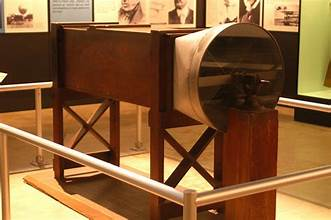
\includegraphics[width=0.6\textwidth]{wind_tunnel.jpg}
	\caption{The Wright Brothers 1901 wind tunnel}
	\label{fig:Wright}
\end{figure}

As computing power increased, designers have leaned more and more towards Computational Fluid Dynamics as a cheaper, faster solution.
The first CFD method was proposed in the 1940s by Lewis Fry Richardson. 
Richardson, a meteorologist, proposed a numerical method for solving partial differential equations to describe fluid flows, but it wasn't until the 1970s and greater computing power that the first CFD software was introduced \cite{resolved_cfd_history}.
With the advent of super computers, engineers can now run simulations previously thought impossible, allowing them to optimize designs.
CFD has led to cheaper and quicker design as engineers can run many simulations at once, instead of having to wait for the results of costly wind tunnel tests.
Even now, engineers are working to improve the existing CFD theories and techniques to further enhance and accelerate simulations.

The classical hydrodynamic theory is one of the foundational theories of CFD \cite{sciencedirect_vortex}. 
It states that fluid flow around a body can be modeled by a distribution of sources, sinks, vortices, and dipoles.
Panel methods take advantage of this theory by defining the surface of the body with a distribution of source panels.
These source panels counter the normal component of the free stream velocity, ensuring the no-flow-through condition.
Here we will derive the panel solve equation for source panels.

% ======================================================
\section{Methods}
The panel method for source panels discretizes the surface of the body into panels, distributing a source to each panel to satisfy the boundary conditions.
For the analysis, we assume that each panel has a constant strength source.
Assuming an inviscid, incompressible, irrotational flow, the following are the governing equations.

\begin{align}
\nabla \cdot \mathbf{u} &= 0, 
&& \text{Incompressible flow}, \\
\nabla \times \mathbf{u} = 0, \; &\Rightarrow \; \mathbf{u} = \nabla \phi,
&& \text{Irrotational flow}, \text{ for some scalar potential $\phi(\mathbf{x})$}, \\
\nabla \cdot (\nabla \phi) &= \nabla^2 \phi = 0, 
&& \text{Substitute into continuity,} \\
\nabla^2 \phi(\mathbf{x}) &= 0, 
&& \text{Laplace's equation}.
\label{eq:basics}
\end{align}

For a body with no-penetration, the surface velocity normal to the surface is zero. This is our boundary condition.
\begin{equation}
\nabla \phi \cdot \mathbf{n} 
\;=\; \mathbf{V}_s \cdot \mathbf{n},
\qquad \text{where $\mathbf{n}$ is the surface normal and $\mathbf{V}_s$ is the surface velocity.}
\label{eq:bc}
\end{equation}

In a 3D source panel method, each panel is assigned a constant source strength $\sigma_j$.
The potential at a point $\mathbf{P}$ is obtained by solving the PDE given by Laplace's equation. 
We know Green's function solves this PDE.
Since we gave each panel a constant strength, we can factor out $\sigma_j$ and find the potential at a point $\mathbf{P}$ of a unit strength source at $\mathbf{Q}$ (\autoref{eq:Greens}).
\begin{align}
G(\mathbf{P},\mathbf{Q}) &= \frac{1}{4\pi r}, 
\quad \text{where } r = \lvert \mathbf{P} - \mathbf{Q} \rvert 
\label{eq:Greens}
\end{align}
\noindent Let $\mathbf{Q}$ and $\mathbf{P}$ be points on the surface $S$.
\vspace{1em}

With Green's function defined, the potential at a field point $\mathbf{P}$ due to all panels can be written as
\begin{equation}
\phi(\mathbf{P}) = \sum_{j=1}^N \sigma_j \int_{S_j} G(\mathbf{P}, \mathbf{Q}) \, dS(\mathbf{Q}),
\label{eq:potential_sum}
\end{equation}
where $\sigma_j$ is the constant source strength on panel $j$.
\vspace{1em}

The velocity is obtained by taking the gradient of the potential,
\begin{equation}
\mathbf{u}(\mathbf{P}) = \nabla_{\mathbf{P}} \phi(\mathbf{P})
= \sum_{j=1}^N \sigma_j \nabla_{\mathbf{P}}
\int_{S_j} G(\mathbf{P}, \mathbf{Q}) \, dS(\mathbf{Q}).
\end{equation}

Applying the no-penetration boundary condition at a control point $\mathbf{P}_i$ on panel $i$ requires
\begin{equation}
\mathbf{u}(\mathbf{P}_i) \cdot \mathbf{n}_i + \mathbf{V}_\infty \cdot \mathbf{n}_i = 0,
\label{eq:boundary}
\end{equation}
where $\mathbf{n}_i$ is the outward surface normal.
\vspace{1em}

We now define the influence coefficient $A_{ij}$ as the induced normal velocity at control point $i$ due to a unit-strength source on panel $j$:
\begin{equation}
A_{ij} = \mathbf{n}_i \cdot \nabla_{\mathbf{P}}
\int_{S_j} G(\mathbf{P}_i, \mathbf{Q}) \, dS(\mathbf{Q}).
\label{eq:Aij_def}
\end{equation}

Evaluating the gradient of the Green’s function gives
\begin{equation}
\nabla_{\mathbf{P}} G(\mathbf{P}, \mathbf{Q})
= - \frac{\mathbf{P} - \mathbf{Q}}{4\pi |\mathbf{P} - \mathbf{Q}|^3}.
\end{equation}

Thus, the influence coefficient for $i\,\neq\,j$ becomes
\begin{equation}
A_{ij} = -\frac{1}{4\pi} \int_{S_j}
\frac{(\mathbf{P}_i - \mathbf{Q}) \cdot \mathbf{n}_i}
{|\mathbf{P}_i - \mathbf{Q}|^3} \, dS(\mathbf{Q}).
\label{eq:Aij_final}
\end{equation}

For $i\,=\,j$, control points lie on the same panel that is acting as the source. 
The limiting value is finite and well-known:
\[\mathbf{A}_{ii} \;=\; -\frac{1}{2}\]

With these equations, we set up a matrix of the influences of every source on every other source using \autoref{eq:Aij_final} giving us an N x N matrix where N is the number of panels.
We factored out the source strength $\sigma_j$ of each panel, giving us a vector of length N. 
And finally, we have our no-flow-through boundary condition from \autoref{eq:bc}, giving us a vector of length N, so we can set up a linear systems of equation. 

\begin{equation}
	\sum_{j=1}^{N} A_{ij} \sigma_j \;=\; -\mathbf{V}_\infty \cdot \mathbf{n}_i
	\label{eq:systems}
\end{equation}

\[
\begin{bmatrix}
A_{11} & \cdots & A_{1N} \\
\vdots & \ddots & \vdots \\
A_{N1} & \cdots & A_{NN} \\
\end{bmatrix}
\begin{bmatrix}
\sigma_1 \\ \vdots \\ \sigma_N
\end{bmatrix}
=
\begin{bmatrix}
\mathbf{V}_\infty \cdot \mathbf{n}_1 \\
\vdots \\
\mathbf{V}_\infty \cdot \mathbf{n}_N \\
\end{bmatrix}
\]

Once we solve the linear systems of equations for $\sigma$, we compute the velocity and coefficient of pressure:
\begin{align}
\mathbf{V}(\mathbf{P}) &= \mathbf{V}_\infty + \sum_{j=1}^{N} \sigma_j \nabla \phi_j (\mathbf{P}) \\
C_p(\mathbf{P}) &= 1 - \frac{\lvert \mathbf{V}(\mathbf{P}) \rvert^2}{\lvert \mathbf{V}_\infty \rvert^2} \\
\label{eq:vel_cp}
\end{align}

% ======================================================
\section{Conclusion}
The panel method is a powerful tool for modeling fluid flow around a body using surface singularities. 
By solving the resulting system, we can find the fluid velocity and pressure distribution without running a full simulation. 
Understanding the derivation and implementation of the source-based panel method provides a strong foundation for future CFD projects in aviation, propulsion, HVAC, and other fields.

% To satisfy the boundary condition, we need the velocity on the surface of the body. 
% Since velocity is the gradient of potential (\autoref{eq:gradient}), to find the velocity at $\mathbf{P}$, we take the gradient of $G(\mathbf{P}, \mathbf{Q})$ w.r.t $\mathbf{P}$.
% \begin{equation}
% \mathbf{u} \;=\; \nabla \phi.
% \label{eq:gradient}
% \end{equation}


\section{References and Resources}

\nocite{*}
\bibliographystyle{new-aiaa}
\bibliography{references}

\end{document}
